\documentclass{beamer} 			
\usepackage[utf8]{inputenc} 
\usepackage[T1]{fontenc}	
\usepackage{lmodern}		
\usepackage[english]{babel}		
\usepackage{amsmath}
\usepackage{amsfonts}
\usepackage{amssymb}
\usepackage{comment}	
\usepackage{epstopdf} 	
\usepackage{bookman}
\usepackage{xcolor}
\usetheme{CambridgeUS}	
\usecolortheme{beaver}		

% Änderungen
\setbeamercovered{transparent}
\setbeamercolor{frametitle}{bg=white}
\setbeamertemplate{frametitle continuation}{}
\setbeamertemplate{navigation symbols}{}	 
\setbeamertemplate{itemize items}{\color{red}$\blacktriangleright$}
%\setbeamertemplate{footline}
\setbeamertemplate{frametitle}
{%
	\vspace{-0.165ex}
	
	\begin{beamercolorbox}[wd=\paperwidth,dp=1ex, ht=6.5ex, sep=0.1ex, colsep*=0pt]{frametitle}%
		\usebeamerfont{frametitle}   \strut \insertframetitle  \\   \usebeamerfont{framesubtitle}   \strut \strut \insertframesubtitle \hfill \raisebox{-4.5ex}[0pt][-\ht\strutbox ]{ 
\includegraphics[width=3cm]{UNSUB.png}}
	\end{beamercolorbox}%
}%

\addtobeamertemplate{title page}{\centering
\includegraphics[scale=0.15]{UNWIDE.png} }{}


\setbeamertemplate{section in toc}[sections numbered]
	
   
\begin{document}
	\title[J.S Industry Characterization]{
	\textbf{A characterization of Colombian industries under Schumpeter's patterns of innovation}
	}   
	\date[BA 2022-30]{Bachelor Thesis. \today} 
	\author[Taborda-Nuñez]{J.~Taborda-Nuñez\inst{1}}
	\institute[Uninorte]{\inst{1}Student. Department of Economics, Universidad del Norte. jtabordaj@uninorte.edu.co}
	\begin{frame} 
		\titlepage 
	\end{frame}  

	\begin{frame}
		\frametitle{Table of Contents}
		\tableofcontents
	\end{frame}


	\AtBeginSection[]
	{
		\begin{frame}
			\frametitle{Table of Contents}
			\tableofcontents[currentsection]
		\end{frame}
	}
	
\section{Introduction}
	\begin{frame}[allowframebreaks]
		\frametitle{Introduction} 
		\begin{itemize}
			\item The question I will answer today is \textbf{Who drives innovation within an industry?}
			\item Could it be a small firm.... Or a large corporation?
			\item \textbf{How?} using Schumpeterian patterns of innovation: \textcolor{red}{Mark I} and \textcolor{blue}{Mark II}
			\item \textbf{Method?} Cluster algorithm
			\item \textbf{Measures?} Three indicators
			\item \textbf{Data sources?} EDIT and EAM surveys
		\end{itemize}
	\end{frame}	
\section{Problem Statement}
	\begin{frame}[allowframebreaks]
		\frametitle{The Problem}
		\begin{itemize}
			\item Characterization exercises "\textit{have been standing the test of time quite well}" (Fontana et al., 2012).
			\item However, no records of said exercises in some countries.
			\item Attempts in Colombia with Schumpeter? \textbf{Yes, but} not in characterization (Umaña-Aponte et al., 2013; Marroquín, 2010; Arroyo-Mina \& Guerrero, 2018; Langebaek-Rueda \& Vásquez, 2007).
			\item Attempts to characterize? \textbf{Yes, but} not with Schumpeter (Cerón et al., 2010; Ovallos-Gazabón \& Amar-Sepúlveda, 2014).
		\end{itemize}
	\end{frame}
	\begin{frame}
		\frametitle{Objectives}
		Main objective: \textbf{characterize} Colombian industries within the manufacturing sectors as Mark I or Mark II industries.
		\begin{itemize}
			\item \textbf{Combine information} from EAM and EDIT
			\item \textbf{Construct quantitative analysis} at the firm level
			\item \textbf{Group industries} through a cluster algorithm
			\item \textbf{Inquire} on potential policy implications
		\end{itemize}
	\end{frame}
\section{Theory and Literature}
	\begin{frame}[allowframebreaks]
		\frametitle{Innovation}
		The concept of innovation:
		\begin{itemize}
			\item \textbf{\textit{"New or improved product or process (or a combination thereof ) that differs
			significantly from the unit's previous products or processes and that has been made available to potential users (product) or brought into use by the unit (process)"}} OECD (2018, p.20)
			\item Innovative activities: Activities to reach innovation
		\end{itemize}
		\framebreak
		Taxonomies of innovation:
		\begin{itemize}
			\item Radical (Schumpeter, 1942): Something new
			\item Incremental (Kirzner, 1973): Enhancements of existing elements
		\end{itemize}
		Other taxonomies (OECD):
		\begin{itemize}
			\item Market, product, process, organizational
		\end{itemize}
	\end{frame}
	\begin{frame}
		\frametitle{Schumpeterian Patterns of Innovation}
		\textcolor{red}{Mark I}
		\begin{itemize}
			\item Small firms are the drivers of innovation (Schumpeter, 1911).
		\end{itemize}
		\textcolor{blue}{Mark II}
		\begin{itemize}
			\item Large firms are the drivers of innovation (Schumpeter, 1942).
		\end{itemize}
	\end{frame}
	\begin{frame}[allowframebreaks]
		\frametitle{Market Structure and Innovation}
		Elements to consider:
		\begin{itemize}
			\item Fontana et al. (2012): Turbulence vs Stability
			\item Arrow replacement effect (1962)
			\item Baumol proposition (2004)
			\item Gilbert (2006) incentives to innovate based on potential profits
			\item Shapiro's revisit (2012): Unifying principle... \textbf{competition}
		\end{itemize}
		\framebreak
		\textcolor{red}{Mark I}
		\begin{itemize}
			\item Perfect competition, \textbf{radical} innovations
		\end{itemize}
		\textcolor{blue}{Mark II}
		\begin{itemize}
			\item Monopoly/Oligopoly, \textbf{incremental} innovations
		\end{itemize}			
	\end{frame}
	\begin{frame}
		\frametitle{Quantification of Schumpeterian Patterns}
		A lot, but mostly:
		\begin{itemize}
			\item \textbf{Stability}
			\item Entry/Exit rate
			\item \textbf{Market Concentration}
			\item Appropriability
			\item \textbf{Technological Opportunities}
		\end{itemize}
	\end{frame}
	\begin{frame}
		\frametitle{Literature}
		Market structure as a determinant of innovation (Loury, 1979; Mansfield, 1963; Raider, 1998)
		\begin{itemize}
			\item Previous characterizations: Malerba and Orsenigo (1996), Breschi et al. (2000), Landström \& Schön (2010), Castellaci and Zheng (2010), Corrocher et al. (2007).
		\end{itemize}
		Two alternatives
		\begin{itemize}
			\item Pavitt: \textbf{Kondratiev waves} (Archibugi, 2001)
			\item Schumpeter: \textbf{Early/Late stages of an industry} (Malerba, 2005)
		\end{itemize}
	\end{frame}
	\begin{frame}
		\frametitle{Colombia's case}
	A periphery economy:
	\begin{itemize}
		\item Dependence Theory (Ahiakpor, 1985)
		\item Empirical evidence sustaining Prebisch-Singer hypothesis (Arezki et al., 2013)
		\item Flows of low/high added value goods
		\item A lot of weight on primary sector, commodities and first gen manufactures
	\end{itemize}
	\end{frame}
\section{Methodology}
	 \begin{frame}
	 	\frametitle{Data sources}
	 	\begin{itemize}
	 		\item Cross-section
	 		\item Inner join of 2018 \textbf{EDIT} ("\textit{Encuesta de Desarrollo
	 		e innovación tecnológica}") and \textbf{EAM} (\textit{Encuesta Anual Manufacturera}) surveys by DANE (2019;2020)
	 		\item EAM is a \textbf{census}; EDIT samples EAM \textbf{industries} --> Inner join
	 		\item Criteria: Employees and profits. Small firms and the informal economy are excluded
	 		\item Each firm has a \textit{"Numero de Orden}" (NORDEMP)
	 		\item Scope: secondary sector, three to four ISIC digits. Initial \textbf{n = 6405}
	 	\end{itemize}
	 \end{frame}
     \begin{frame}[allowframebreaks]
     	\frametitle{Dimensions}
     	Concentration (\textit{CON}):
     	\begin{itemize}
     		\item Malerba and Orsenigo (1996)
     		\item H-H Concentration Index of Market Share of output, innovative activities, labour demand and supply
     		\item Geometrical mean
     	\end{itemize} 
     	\begin{equation}
     		\centering
     		CON = (HH_{ms}*HH_{msa}*HH_{lsd}*HH_{ss})^{1/4}
     	\end{equation}
     \framebreak
     
     Technological Opportunities (\textit{TO})
     \begin{itemize}
     	\item Maleki et al. (2018)
     	\item Relative change of protection mechanisms 
     	\item Conventional and non-conventional
     \end{itemize}
 	 \begin{equation}
 	 \centering
 	 TO = \dfrac{PM_{1718} + NCPM_{1718}}{PM}
 	 \end{equation}
  	\framebreak
  	
  	Stability (\textit{STA})
  	\begin{itemize}
  		\item The dynamic problem.\textbf{ EDIT is non comparable}
  		\item Thus, we need another approach. A static approach
  		\item Based on Baumol (2004) proposition
  	\end{itemize}
  		\begin{equation}
  		\centering
  		STA = Sr - Si
  		\end{equation}
\end{frame}
\section{The Cluster}
	\begin{frame}
		\frametitle{Warming up}
		\begin{itemize}
			\item Some data limitations --> Data availability
			\item Some industries report zero innovation spending, or have a small amount of firms
			\item Filter for industries with less than 20 firms. Resulting \textbf{n = 5986}
			\item k-means cluster --> Lloyd algorithm and 10 repetitions
		\end{itemize}
	\end{frame}
	\begin{frame}
		\begin{figure}[H]	
			\caption{Preliminary characterization of Colombian Manufacture using a two groups k-means clustering method}
			\centering
			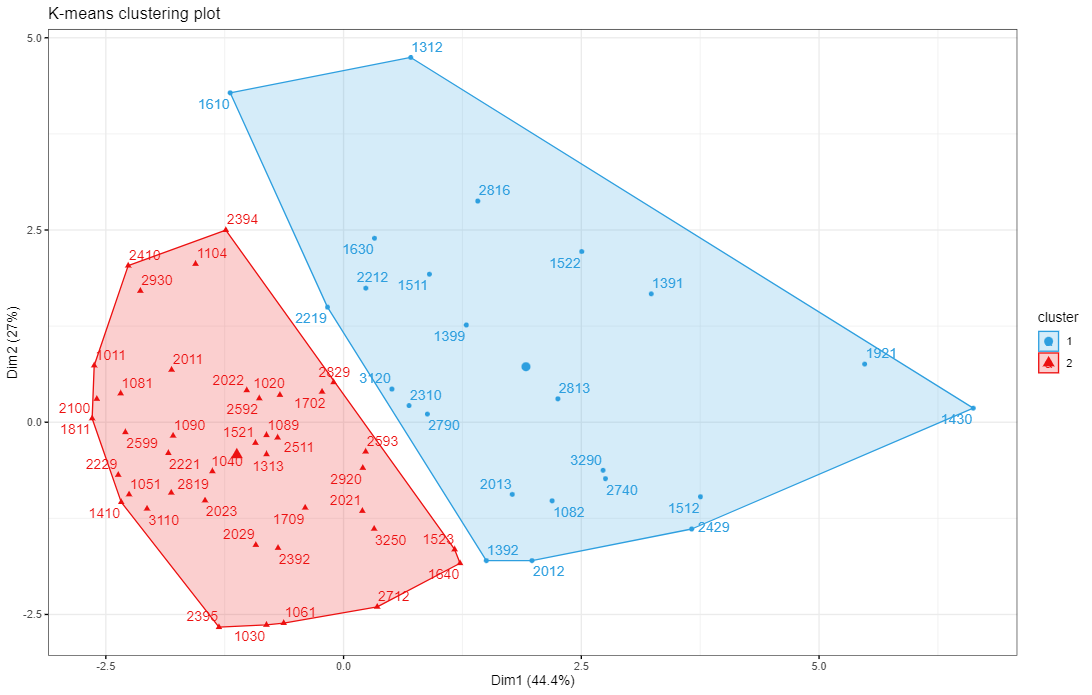
\includegraphics[scale = 0.29]{cluster.png}
		\end{figure}
	\end{frame} 
	\begin{frame}
	\frametitle{Results}
	\begin{itemize}
		\item Dim1 and Dim2
		\item Two groups: Cluster Group 1 (CG1) and Cluster Group 2 (CG2)
		\begin{itemize}
			\item \textcolor{blue}{CG1} --> n = 794
			\item \textcolor{red}{CG2}  --> n = 5192
		\end{itemize}
	\end{itemize}
	\end{frame}

	\begin{frame}[allowframebreaks]
	\begin{figure}
		\centering
		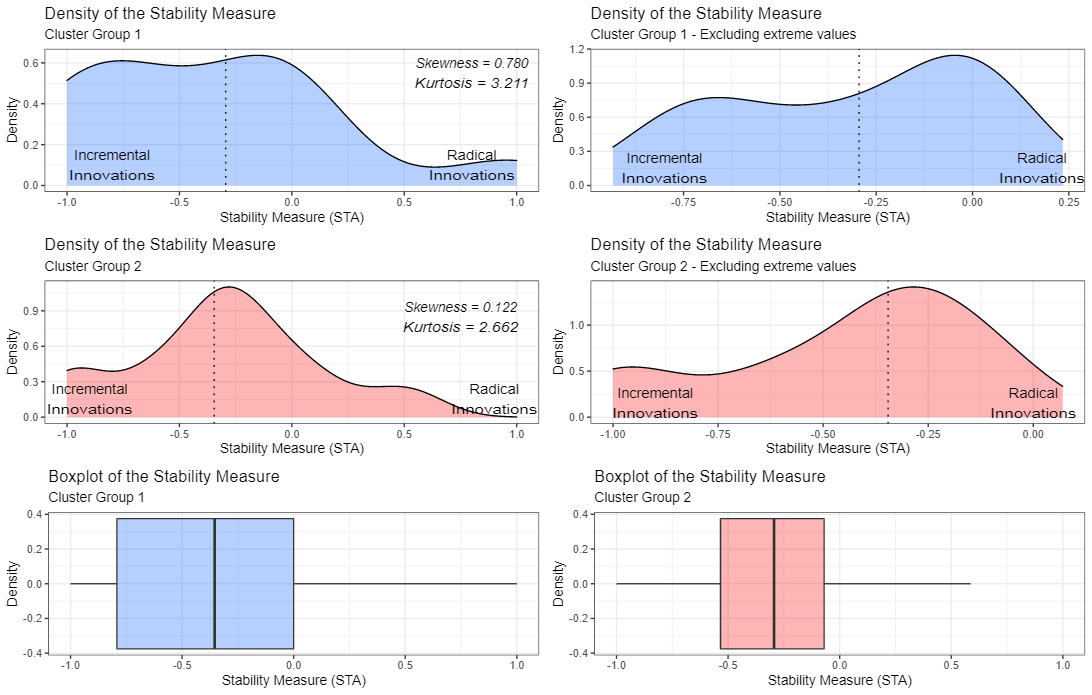
\includegraphics[scale=0.30]{sta.png}
	\end{figure}
	\framebreak
	\begin{figure}
		\centering
		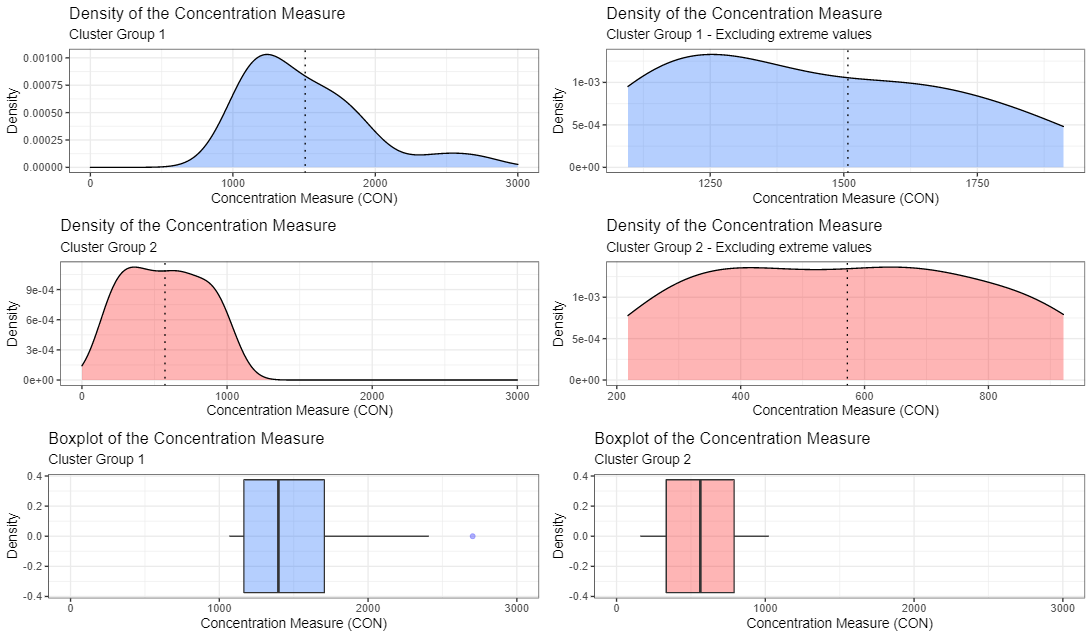
\includegraphics[scale=0.31]{pcon.png}
	\end{figure}
	\framebreak
	\begin{figure}
		\centering
		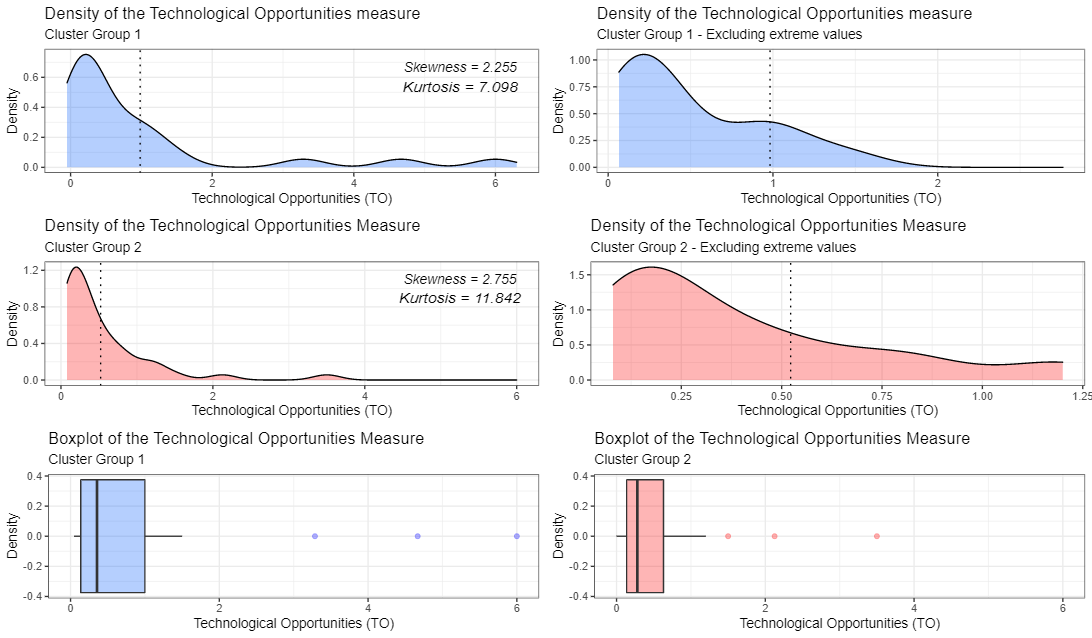
\includegraphics[scale=0.31 ]{to.png}
	\end{figure}
	\framebreak
	\end{frame}
\section{Implications}
	\begin{frame}
		\frametitle{General Implications}
		\textbf{The most important implication:}
		\begin{itemize}
			\item \textbf{\textcolor{red}{Red cluster}} (CG2): Mark I industries, small firms drive innovation
			\item \textbf{\textcolor{blue}{Blue cluster}} (CG1): Mark II industries, large firms drive innovation
		\end{itemize}
	\end{frame}
	\begin{frame}[allowframebreaks]
		\frametitle{Policy implications}
		Several implications for certain segments:
		\begin{itemize}
			\item \textbf{\textcolor{green}{Groceries, meat, coffee}}: Mark I. \textbf{Exception} in \textbf{\textcolor{brown}{Chocolates.}} (\textit{Nutresa?})
			\item \textbf{\textcolor{teal}{First-gen manufacture}}: Mark II. \textbf{Exception} in \textbf{\textcolor{gray}{Elaboration and finishing of clothing}}
			\item \textbf{\textcolor{olive}{Petroleum}}: Mark II (\textit{Ecopetrol?})
			\item \textbf{\textcolor{orange}{Furnitures and wood products}}: Mixed results
			\item \textbf{\textcolor{lightgray}{Metals and minerals}}: Mixed results, but more complex minerals/metals as Mark II
		\end{itemize}
		\framebreak
		Policy guidelines:
		\begin{itemize}
			\item Differentiated approach
			\item Identify strategic sectors
			\item Incentive architecture around flagships
			\item Domino-effects and chained sectors
			\item Goods as final goods, or as inputs?
		\end{itemize}
	\end{frame}
\section{Conclusions}
	\begin{frame}[allowframebreaks]
		\frametitle{Conclusions}
		Some broad conclusions:
		\begin{itemize}
			\item We have been able to \textbf{characterize} industries. Schumpeterian patterns persist
			\item We found \textbf{who drives innovation} across CG1 and CG2
			\item Concentration is the spearhead of the study
			\item But other dimensions also shed light!
			\item Policy implications... not one size fits all, context matter, strategic sectors need strategic solutions, focus on incentives.
			\framebreak
			\item Some limitations... we can extend based on this work
			\item Include static components, the \textbf{how} of incentives and future econometric approaches
		\end{itemize}
	\end{frame}
\end{document}